\chapter{Transistor BJT}

\renewcommand\thesection{\Roman{section}}

\textbf{Obiettivo:} ricavare la caratteristica in uscita ed in ingresso del transistor BJT.

\paragraph{Strumentazione:} 
\begin{enumerate}
    \item due generatori di tensione;
    \item un transistor BJT;
    \item una resistenza $R_b$ da $\SI{10}{\kilo\Omega}$;
    \item due amperometri e due voltmetri.
\end{enumerate}

\paragraph{Procedura:}
\begin{enumerate}
    \item costruire il circuito;
    \begin{figure}[h]
        \centering
        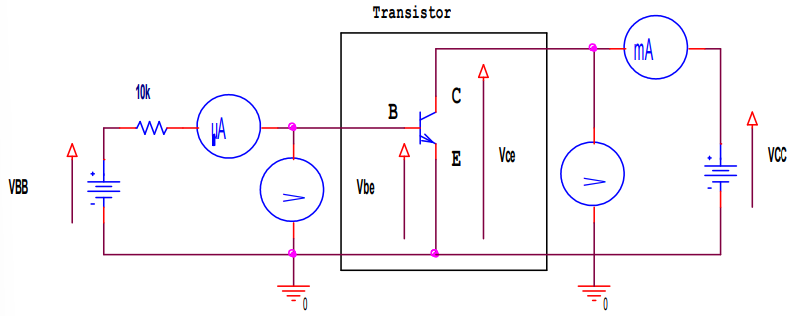
\includegraphics[width=0.75\linewidth]{Immagini/EXP6 - IV BJT.png}
        \caption{circuito per la I-V del BJT.}
        \label{fig: EXP6 - IV BJT}
    \end{figure}
    \item per evitare che le caratteristiche siano compromesse dall'aumento della temperatura del transistor è necessario limitare la potenza dissipata. A tal fine è necessario disegnare, prima di iniziare le misure, la curva di massima potenza: $P_{max} = V_{ce}I_c$ che nel piano $I_c = f(V_{ce})$ è rappresentata da un iperbole. Il transistor del laboratorio è del tipo NPN con sigla TIP31 e può dissipare al massimo $\SI{1}{\watt}$;
    \item variando $V_{be}$ tramite $V_{bb}$, impostare una corrente di base di $\SI{100}{\micro\ampere}$;
    \item leggere la tensione $V_{be}$;
    \item variare la tensione $V_{ce}$ (registrarla) tramite $V_{cc}$ e leggere la corrente $I_c$. Annotarsi la corrente $I_b$ e la tensione $V_{be}$ ad ogni variazione di $V_{ce}$. Se la corrente $I_b$ dovesse variare per un certo valore di $V_{ce}$ (quando si passa da regione di saturazione a regione attiva) non reimpostare $V_{be}$.
    \item si ripete la procedura variando la corrente $I_b$ da $\SI{100}{\micro\ampere}$ a $\SI{400}{\micro\ampere}$ a passi di $\SI{50}{\micro\ampere}$, così da ricavare la famiglia di curve $I_c=f(V_{ce})$ per $I_b=costante$;
    \item si ricavi inoltre la famiglia $I_b=f(V_{be})$ con $V_{ce}=costante$ e $\beta_f=I_c/I_b=f(I_c)$ per $V_{ce}=\SI{6}{\volt}$;
    \item si ricavi infine la tensione di Early effettuando una regressione lineare delle curve $I_c=f(V_{ce})$ nella regione attiva.
\end{enumerate}

\setcounter{section}{0}
\renewcommand\thesection{\Alph{section}}

\section{Effetto Early}
L'effetto Early si riferisce alla variazione di $I_c$ con la variazione della tensione $V_{ce}$, anche quando $I_b$ è costante. Idealmente, ci si aspetterebbe che $I_c$ sia indipendente da $V_{ce}$ nella regione attiva del BJT, ma in pratica $I_c$ tende ad aumentare con $V_{ce}$. Questo avviene perché l'area della regione base-collettore si riduce leggermente con l'aumentare di $V_{ce}$, riducendo la probabilità di ricombinazione e quindi provocando un aumento di $I_c$.

La tensione di Early $V_A$ è un parametro che quantifica l'effetto Early. Può essere interpretata come il valore ipotetico di $V_{ce}$ per cui $I_c$ si annullerebbe. La tensione di Early è normalmente negativa dato che l'inclinazione delle rette $I_c=f(V_{ce})$ è molto contenuta.